% Created 2019-05-23 Thu 06:14
% Intended LaTeX compiler: pdflatex
\documentclass[10pt,oneside,x11names]{article}
\usepackage[utf8]{inputenc}
\usepackage[T1]{fontenc}
\usepackage{graphicx}
\usepackage{grffile}
\usepackage{longtable}
\usepackage{wrapfig}
\usepackage{rotating}
\usepackage[normalem]{ulem}
\usepackage{amsmath}
\usepackage{textcomp}
\usepackage{amssymb}
\usepackage{capt-of}
\usepackage{hyperref}
\usepackage{amsmath}
\usepackage{interval}  % must install texlive-full
\usepackage[shortcuts]{extdash}
\usepackage[top=0.90in,bottom=0.55in,left=1in,right=1in,includefoot]{geometry}
\usepackage{palatino}
\usepackage{siunitx}
\usepackage{braket}
\usepackage[euler-digits,euler-hat-accent]{eulervm}
\usepackage{fancyhdr}
\pagestyle{fancyplain}
\lhead{}
\chead{Confidential The TBD Group 2019}
\rhead{}
\lfoot{Confidential The TBD Group 2019}
\cfoot{\thepage}
\rfoot{}
\usepackage{lineno}
\linenumbers
\newcommand\definedas{\stackrel{\text{\tiny def}}{=}}
\usepackage{mdframed}
\BeforeBeginEnvironment{minted}{\begin{mdframed}}
\AfterEndEnvironment{minted}{\end{mdframed}}
\author{Brian Beckman}
\date{\today}
\title{Composable Statistics}
\hypersetup{
 pdfauthor={Brian Beckman},
 pdftitle={Composable Statistics},
 pdfkeywords={},
 pdfsubject={},
 pdfcreator={Emacs 26.2 of 2019-04-12, org version: 9.2.2},
 pdflang={English}}
\begin{document}

\maketitle
\setcounter{tocdepth}{2}
\tableofcontents


\section{COMPOSABLE STATISTICS}
\label{composable-statistics}
\subsection{{\bfseries\sffamily TODO} TANGLE, NOWEB}
\label{sec:orgdcdc907}

This will become a fully literate program via org-babel \texttt{tangle} and
\texttt{noweb}. At present, it is an org file converted directly from an old
iPython (Jupyter) notebook. Jupyter proved not to scale well.

\subsection{{\bfseries\sffamily TODO} GRAPHICS}
\label{sec:org2a3cef0}

We still
have to work out how to embed graphics in this file.

\subsection{CLOJURE}
\label{clojure}
We prefer Clojure to Python for this exercise due to Clojure's
concurrency primitives, especially atoms and core.async. Python is
growing and improving rapidly, so we may return to it someday.

\subsubsection{{\bfseries\sffamily TODO} PROJECT.CLJ}
\label{sec:orgac402ea}

At present, the critical file \texttt{project.clj} is external to this
document. It will be one of the first to tangle.

The best sites for learning Clojure by example are
\href{http://clojuredocs.org}{clojuredocs.org} and
\href{http://4clojure.org}{4clojure.org}. A recommended book is
\href{http://braveclojure.com}{Clojure for the Brave and True}.

\subsection{{\bfseries\sffamily TODO} HOW TO USE THIS DOCUMENT}
\label{how-to-use-this-document}
Explain how to run Clojure code inside an org-mode buffer, how to tangle and
weave, etc.

\begin{enumerate}
\item Install leiningen \url{https://leiningen.org/} (this is all you need for Clojure)
\end{enumerate}

\section{INTRODUCTION}
\label{introduction}
We want to compute descriptive statistics in constant memory. We want
exactly the same code to run over sequences distributed in space as runs
over sequences distributed in time. Sequences distributed in space are
vectors, lists, arrays, lazy or not. Sequences distributed over time are
asynchronous streams. Descriptive statistics range from \texttt{count}, \texttt{mean},
\texttt{max}, \texttt{min}, and \texttt{variance} to Kalman filters and Gaussian processes.
We decouple computation from data delivery by packaging computation in
composable functions.

Some sample scalar data:

\begin{verbatim}
(def zs [-0.178654, 0.828305, 0.0592247, -0.0121089, -1.48014,
         -0.315044, -0.324796, -0.676357, 0.16301, -0.858164])
\end{verbatim}

\subsection{TODO: GENERATE NEW RANDOM DATA}
\label{sec:org74463e6}

\section{RUNNING COUNT}
\label{running-count}
The traditional and obvious way with \texttt{reduce} and \texttt{reductions}
(\url{https://clojuredocs.org/clojure.core/reduce}). \emph{Reduce} takes three
arguments: a binary function, an initial value, and a space-sequence of
inputs.

\begin{verbatim}
(reduce
    (fn [count datum] (inc count)) ; binary function
    0                              ; initial value
    zs)                            ; space sequence
\end{verbatim}

\begin{verbatim}
10
\end{verbatim}


\ldots{} with all intermediate results:

\begin{verbatim}
(reductions (fn [c z] (inc c)) 0 zs)
\end{verbatim}

\begin{center}
\begin{tabular}{rrrrrrrrrrr}
0 & 1 & 2 & 3 & 4 & 5 & 6 & 7 & 8 & 9 & 10\\
\end{tabular}
\end{center}

\subsection{THREAD-SAFE}
\label{thread-safe}
Overkill for sequences in space, but safe for multiple threads from
asynchronous streams. It also shows (1) \emph{let-over-lambda} (LOL): closing
over mutable state variables, and (2) transactional mutation, i.e.,
\emph{atomic updates}. LOL is sematically equivalent to data encapsulation in
OOP, and transactions are easier to verify than is OOP with locks and
mutexes.

The following has a defect: we need \texttt{initial-count} both to initialize
the atom and to initialize the \texttt{reduce} call. This defect must be traded
off against the generalizable form or \emph{functional type} of the
reducible, namely
\((\textrm{estimate}, \textrm{measurement})\rightarrow\textrm{estimate}\).
We get rid of this defect later.

\begin{verbatim}
(let [initial-count 0] ; Must use this twice below.
    (reduce
        ; Let-over-lambda (anonymous "object") follows.
        ; "Atom" is a transactional (thread-safe) type in Clojure.
        (let [running-count (atom initial-count)]
            ; That was the "let" of "LOL." Here comes the lambda:
            ; Reducible closure over "running-count."
            (fn [c z] ; Here's the "lambda" of "LOL"
                (swap! running-count inc) ; transactional update
                @running-count))
                ; safe "read" of the atom ~~> new value for c
        initial-count
        zs))
\end{verbatim}

\begin{verbatim}
10
\end{verbatim}


Showing all intermediate results:

\begin{verbatim}
(let [initial-count 0]
    (reductions ; <-- this is the only difference to above
        (let [running-count (atom initial-count)]
            (fn [c z]
                (swap! running-count inc)
                @running-count)) ; ~~> new value for c
        initial-count
        zs))
\end{verbatim}

\begin{center}
\begin{tabular}{rrrrrrrrrrr}
0 & 1 & 2 & 3 & 4 & 5 & 6 & 7 & 8 & 9 & 10\\
\end{tabular}
\end{center}

\subsection{AVOIDING \emph{REDUCE}}
\label{avoiding-reduce}
\texttt{Reduce} only works in space, not in time. Avoiding \texttt{reduce} decouples
the statistics code (``business logic'') from the space environment
(``plumbing''). That spaces environment delivers data from vectors, lists,
etc.). We want to be able to switch out an environment that delivers
data from space for an environment that delivers data points \(z\) from
time.

The following is a thread-safe LOL, without \texttt{reduce}. We \emph{map} the LOL
over a space-sequence in memory to produce exactly the same result as
with \texttt{reduce}. The mappable LOL does not need an accumulator argument
for \texttt{count}.

Below, we map \emph{exactly} the same mappable LOL over asynchronous streams.

A subtle defect: the output is still coupled to the computing
environment through \texttt{print}. We get rid of that, too,
\hyperref[REMOVING-OUTPUT-COUPLING]{below}.

\begin{verbatim}
(dorun ; <-- Discard 'nil's produced by "print."
    (map
        (let [running-count (atom 0)]
            (fn [z] ; <-- one fewer argument
                (swap! running-count inc)
                (print (str @running-count " "))))
        zs))
\end{verbatim}

\begin{verbatim}
1 2 3 4 5 6 7 8 9 10
\end{verbatim}

\section{RUNNING MEAN}
\label{running-mean}
Consider the following general scheme for recurrence: \textbf{\emph{a new statistic is an
old statistic plus a correction}}.

The \emph{correction} is a \emph{gain} times a \emph{residual}. For running mean, the
residual is the difference between the new measurement \(z\) and the old
mean \(x\). The gain is \(1/(n+1)\), where \(n\) is \emph{count-so-far}. \(n\) is a
statistic, too, so it is an \emph{old} value, computed and saved before the
current observation \(z\) arrived.

/The correction therefore depends only on the new input \(z\) and on old
statistics \(x\) and \(n\). The correction does not depend on new
statistics/.

Mathematically, write the general recurrence idea without subscripts as

$$x\leftarrow{x+K\,(z-x)}$$

or, with Lamport's notation, wherein new versions of old values get a
prime, as an equation

$$x'=x+K\,(z-x)$$

(\(z\) does not have a prime; it is the only exception to the rule that
new versions of old quantities have primes).

Contrast the noisy traditional form, which introduces another variable,
the index \(n\). This traditional form is objectively more complicated
than either of the two above:

$$x_{n+1}=x_n+K(n)\,(z_{n+1}-x_n)$$

\begin{verbatim}
(dorun
    (map
        (let [running-stats (atom {:count 0, :mean 0})]
            (fn [z]
                (let [{x :mean, n :count} @running-stats
                      n+1 (inc n) ; cool variable name!
                      K   (/ 1.0 n+1)]
                    (swap! running-stats conj
                           [:count n+1]
                           [:mean (+ x (* K (- z x)))]))
                (println @running-stats)))
        zs))
\end{verbatim}

\begin{verbatim}
{:count 1, :mean -0.178654}
{:count 2, :mean 0.3248255}
{:count 3, :mean 0.2362919}
{:count 4, :mean 0.1741917}
{:count 5, :mean -0.15667464000000003}
{:count 6, :mean -0.18306953333333337}
{:count 7, :mean -0.20331617142857145}
{:count 8, :mean -0.262446275}
{:count 9, :mean -0.21517335555555556}
{:count 10, :mean -0.27947242}
\end{verbatim}

The \texttt{swap} above calls \texttt{conj} on the current contents of the atom
\texttt{running-stats} and on the rest of the arguments, namely
\texttt{[:count n+1, :mean ...]}. \texttt{conj} is the idiom for ``updating'' a hashmap,
the hashmap in the atom, the hashmap that starts off as
\texttt{\{:count 0, :mean 0\}}.

\subsection{REMOVING OUTPUT COUPLING}
\label{REMOVING-OUTPUT-COUPLING}
Remove \texttt{println} from inside the LOL function of \(z\). Now the LOL
function of \(z\) is completely decoupled from its environment. Also,
abstract a ``factory'' method for the LOL, \emph{make-running-stats-mapper}, to
clean up the line that does the printing.

\subsubsection{MAKE-RUNNING-STATS-MAPPER}
\label{make-running-stats-mapper}
\begin{verbatim}
(defn make-running-stats-mapper []
    (let [running-stats (atom {:count 0 :mean 0 :datum 0})]
        (fn [z]
            (let [{x :mean, n :count, _ :datum} @running-stats
                  n+1 (inc n)
                  K   (/ 1.0 n+1)]
                (swap! running-stats conj
                       [:count n+1]
                       [:mean (+ x (* K (- z x)))]
                       [:datum z]))
            @running-stats)))

(clojure.pprint/pprint (map (make-running-stats-mapper) zs))
\end{verbatim}

\begin{verbatim}
({:count 1, :mean -0.178654, :datum -0.178654}
 {:count 2, :mean 0.3248255, :datum 0.828305}
 {:count 3, :mean 0.2362919, :datum 0.0592247}
 {:count 4, :mean 0.1741917, :datum -0.0121089}
 {:count 5, :mean -0.15667464000000003, :datum -1.48014}
 {:count 6, :mean -0.18306953333333337, :datum -0.315044}
 {:count 7, :mean -0.20331617142857145, :datum -0.324796}
 {:count 8, :mean -0.262446275, :datum -0.676357}
 {:count 9, :mean -0.21517335555555556, :datum 0.16301}
 {:count 10, :mean -0.27947242, :datum -0.858164})
\end{verbatim}

\subsection{NUMERICAL CHECK}
\label{numerical-check}
The last value of the running mean is \(-0.279...42\). Check that against
an independent calculation.

\begin{enumerate}
\item DEFN MEAN
\label{sec:orgec8f1cb}

\begin{verbatim}
(defn mean [zs] (/ (reduce + zs) (count zs)))
(println (mean zs))
\end{verbatim}

\begin{verbatim}
-0.27947242
\end{verbatim}
\end{enumerate}

\section{CORE.ASYNC}
\label{core.async}
For data distributed over time, we'll use Clojure's core.async.
Core.async has some subtleties that we analyze below.

\begin{verbatim}
(require
    '[clojure.core.async
      :refer
      [sliding-buffer dropping-buffer buffer
       <!!,  <!,  >!,  >!!,
       go chan onto-chan close!
       thread alts! alts!! timeout]])
\end{verbatim}

\subsection{SHALLOW TUTORIAL}
\label{shallow-tutorial}
\url{https://github.com/clojure/core.async/blob/master/examples/walkthrough.clj}

\subsection{DEEP TUTORIAL}
\label{deep-tutorial}
The asynchronous, singleton \texttt{go} thread is loaded with very lightweight
\emph{pseudothreads} (my terminology, not standard; most things you will read
or see about Clojure.async does not carefully distinguish between
threads and pseudothreads, and I think that's not helpful).

Pseudothreads are lightweight state machines that pick up where they
left off. It is feasible to have thousands, even millions of them.
Pseudothreads don't block, they \emph{park}. \emph{Parking} and \emph{unparking} are
very fast. We can write clean code with pseudothreads because our code
looks like it's blocked waiting for input or blocked waiting for buffer
space. Code with blocking I/O is easy to write and to understand. Code
in \texttt{go} forms doesn't actually block, just looks like it.

Some details are tricky and definitely not easy to divine from the
documentation. Hickey's video from InfoQ 2013
(\url{https://www.infoq.com/presentations/core-async-clojure}) is more
helpful, but you can only appreciate the fine points after you've
stumbled a bit. I stumbled over the fact that buffered and unbuffered
channels have different synchronization semantics. Syntactically, they
look the same, but you cannot, in general, run the same code over an
unbuffered channel that works on a buffered channel. Hickey says this,
but doesn't nail it to the mast; doesn't emphasize it with an example,
as I do here in this deep tutorial. He motivates the entire library with
the benefits of first-class queues, but fails to emphasize that, by
default, a channel is not a queue but a blocking rendezvous. He does
mention it, but one cannot fully appreciate the ramifications from a
passing glance.

\subsubsection{COMMUNICATING BETWEEN THREADS AND PSEUDOTHREADS}
\label{communicating-between-threads-and-pseudothreads}
Write output to unbuffered channel \texttt{c} via \texttt{>!} on the asynchronous \texttt{go}
real-thread and read input from the same channel \texttt{c} via \texttt{<!!} on the
UI/REPL \texttt{println} real-thread. We'll see later that writing via \texttt{>!!} to
an unbuffered channel blocks the UI real-thread, so we can't write
before reading unbuffered on the UI/REPL real-thread. However, we can
write before reading on a non-blocking pseudothread, and no buffer space
is needed.

\begin{verbatim}
(let [c (chan)]        ;; unbuffered chan
    (go (>! c 42))     ;; parks if no space in chan
    (println (<!! c))  ;; blocks UI/REPL until data on c
    (close! c))        ;; idiom; may be harmless overkill
\end{verbatim}

\begin{verbatim}
42
\end{verbatim}


In general, single-bang forms work on \texttt{go} pseudothreads, and
double-bang forms work on real, heavyweight, Java threads like the
UI/REPL thread behind this notebook. In the rest of this notebook,
``thread'' means ``real thread'' and we write ``pseudothread'' explicitly when
that's what we mean.

I don't address thread leakage carefully in this tutorial, mostly
because I don't yet understand it well. I may overkill by closing
channels redundantly.

\subsubsection{CHANNEL VOODOO FIRST}
\label{channel-voodoo-first}
Writing before reading seems very reasonable, but it does not work on
unbuffered channels, as we see below. Before going there, however, let's
understand more corners of the example above.

The \texttt{go} form itself returns a channel:

\begin{verbatim}
(clojure.repl/doc go)
\end{verbatim}

\begin{verbatim}
-------------------------
clojure.core.async/go
([& body])
Macro
  Asynchronously executes the body, returning immediately to the
  calling thread. Additionally, any visible calls to <!, >! and alt!/alts!
  channel operations within the body will block (if necessary) by
  'parking' the calling thread rather than tying up an OS thread (or
  the only JS thread when in ClojureScript). Upon completion of the
  operation, the body will be resumed.

  Returns a channel which will receive the result of the body when
  completed
\end{verbatim}

I believe ``the calling thread'' above refers to a pseudothread inside the
\texttt{go} real-thread, but I am not sure because of the ambiguities in the
official documentation between ``blocking'' and ``parking'' and between
``thread'' and ``well, we don't have a name for them, but Brian calls them
`pseudothreads'.''

Is the channel returned by \texttt{go} the same channel as \texttt{c}?

\begin{verbatim}
(let [c (chan)]
    (println {:c-channel c})
    (println {:go-channel (go (>! c 42))})
    (println {:c-coughs-up (<!! c)})
    (println {:close-c (close! c)}))
\end{verbatim}

\begin{verbatim}
{:c-channel #object[clojure.core.async.impl.channels.ManyToManyChannel 0x2e16e617 clojure.core.async.impl.channels.ManyToManyChannel@2e16e617]}
{:go-channel #object[clojure.core.async.impl.channels.ManyToManyChannel 0x54f4c749 clojure.core.async.impl.channels.ManyToManyChannel@54f4c749]}
{:c-coughs-up 42}
{:close-c nil}
\end{verbatim}


No, \texttt{c} is a different channel from the one returned by \texttt{go}. Consult
the documentation for \texttt{go} once more:

\begin{verbatim}
(clojure.repl/doc go)
\end{verbatim}

\begin{verbatim}
-------------------------
clojure.core.async/go
([& body])
Macro
  Asynchronously executes the body, returning immediately to the
  calling thread. Additionally, any visible calls to <!, >! and alt!/alts!
  channel operations within the body will block (if necessary) by
  'parking' the calling thread rather than tying up an OS thread (or
  the only JS thread when in ClojureScript). Upon completion of the
  operation, the body will be resumed.

  Returns a channel which will receive the result of the body when
  completed
\end{verbatim}

We should be able to read from the channel returned by \texttt{go}; call it
\texttt{d}:

\begin{verbatim}
(let [c (chan)
      d (go (>! c 42))] ;; 'let' in Clojure is sequential,
                        ;; like 'let*' in Scheme or Common Lisp,
                        ;; so 'd' has a value, here.
    (println {:c-coughs-up (<!! c),  ;; won't block
              :d-coughs-up (<!! d)}) ;; won't block
    (close! c)
    (close! d))
\end{verbatim}

\begin{verbatim}
{:c-coughs-up 42, :d-coughs-up true}
\end{verbatim}


\texttt{d}'s coughing up \texttt{true} means that the body of the \texttt{go}, namely
\texttt{(>! c 42)} must have returned \texttt{true}, because \texttt{d} coughs up ``the result
of the body when completed.'' Let's see whether our deduction matches
documentation for \texttt{>!}:

\begin{verbatim}
(clojure.repl/doc >!)
\end{verbatim}

\begin{verbatim}
-------------------------
clojure.core.async/>!
([port val])
  puts a val into port. nil values are not allowed. Must be called
  inside a (go ...) block. Will park if no buffer space is available.
  Returns true unless port is already closed.
\end{verbatim}


Sure enough. But something important is true and not obvious from this
documentation. Writing to \texttt{c} inside the \texttt{go} block parks the
pseudothread because no buffer space is available: \texttt{c} was created with
a call to \texttt{chan} with no arguments, so no buffer space is allocated.
Only when reading from \texttt{c} does the pseudothread unpark. How? There is
no buffer space. Reading on the UI thread manages to short-circuit any
need for a buffer and unpark the pseudothread. Such short-circuiting is
called a \emph{rendezvous} in the ancient literature of concurrency. Would
the pseudothread unpark if we read inside a \texttt{go} block and not on the UI
thread?

\begin{verbatim}
(let [c (chan)
      d (go (>! c 42))
      e (go (<! c))]
    (clojure.pprint/pprint {
      :c-channel c, :d-channel d, :e-channel e,
      :e-coughs-up (<!! e),  ;; won't block
      :d-coughs-up (<!! d)}) ;; won't block
    (close! c)
    (close! d)
    (close! e))
\end{verbatim}

\begin{verbatim}
{:c-channel
 #object[clojure.core.async.impl.channels.ManyToManyChannel 0xef5b34a "clojure.core.async.impl.channels.ManyToManyChannel@ef5b34a"],
 :d-channel
 #object[clojure.core.async.impl.channels.ManyToManyChannel 0x7cad6aee "clojure.core.async.impl.channels.ManyToManyChannel@7cad6aee"],
 :e-channel
 #object[clojure.core.async.impl.channels.ManyToManyChannel 0x44a336e2 "clojure.core.async.impl.channels.ManyToManyChannel@44a336e2"],
 :e-coughs-up 42,
 :d-coughs-up true}
\end{verbatim}


Yes, the pseudothread that parked when \(42\) is put on \texttt{c} via \texttt{>!}
unparks when \(42\) is taken off via \texttt{<!}. Channel \texttt{d} represents the
parking step and channel \texttt{e} represents the unparking step. All three
channels are different.

So now we know how to short-circuit or rendezvous unbuffered channels.
In fact, the order of reading and writing (taking and putting) does not
matter in the nebulous, asynchronous world of pseudothreads. How
Einsteinian is that? The following takes (reads) from \texttt{c} on \texttt{e} before
puting (writing) to \texttt{c} on \texttt{d}. That's the same as above, only in the
opposite order.

\begin{verbatim}
(let [c (chan)
      e (go (<! c))
      d (go (>! c 42))]
    (clojure.pprint/pprint {
      :c-channel c, :d-channel d, :e-channel e,
      :e-coughs-up (<!! e),  ;; won't block
      :d-coughs-up (<!! d)}) ;; won't block
    (close! c)
    (close! d)
    (close! e))
\end{verbatim}

\begin{verbatim}
{:c-channel
 #object[clojure.core.async.impl.channels.ManyToManyChannel 0x53929fdb "clojure.core.async.impl.channels.ManyToManyChannel@53929fdb"],
 :d-channel
 #object[clojure.core.async.impl.channels.ManyToManyChannel 0x5cdd3796 "clojure.core.async.impl.channels.ManyToManyChannel@5cdd3796"],
 :e-channel
 #object[clojure.core.async.impl.channels.ManyToManyChannel 0xe214199 "clojure.core.async.impl.channels.ManyToManyChannel@e214199"],
 :e-coughs-up 42,
 :d-coughs-up true}
\end{verbatim}

\subsubsection{PUTS BEFORE TAKES CONSIDERED RISKY}
\label{puts-before-takes-considered-risky}
\texttt{>!!}, by default, blocks if called too early on an unbuffered real
thread. We saw above that parked pseudothreads don't block: you can read
and write to channels in \texttt{go} blocks in any order. However, that's not
true with threads that actually block. The documentation is obscure,
though not incorrect, about this fact.

\begin{verbatim}
(clojure.repl/doc >!!)
\end{verbatim}

\begin{verbatim}
-------------------------
clojure.core.async/>!!
([port val])
  puts a val into port. nil values are not allowed. Will block if no
  buffer space is available. Returns true unless port is already closed.
\end{verbatim}


When is ``no buffer space available?'' It turns out that the default
channel constructor makes a channel with no buffer space allocated by
default.

\begin{verbatim}
(clojure.repl/doc chan)
\end{verbatim}

\begin{verbatim}
-------------------------
clojure.core.async/chan
([] [buf-or-n] [buf-or-n xform] [buf-or-n xform ex-handler])
  Creates a channel with an optional buffer, an optional transducer
  (like (map f), (filter p) etc or a composition thereof), and an
  optional exception-handler.  If buf-or-n is a number, will create
  and use a fixed buffer of that size. If a transducer is supplied a
  buffer must be specified. ex-handler must be a fn of one argument -
  if an exception occurs during transformation it will be called with
  the Throwable as an argument, and any non-nil return value will be
  placed in the channel.
\end{verbatim}

We can test the blocking-on-unbuffered case as follows. The following
code will block at the line \texttt{(>!! c 42)}, as you'll find if you
uncomment the code (remove \texttt{\#\_} at the beginning) and run it. You'll
have to interrupt the Kernel using the ``Kernel'' menu at the top of the
notebook, and you might have to restart the Kernel, but you should try
it once.

\begin{verbatim}
#_(let [c (chan)]
    (>!! c 42)
    (println (<!! c))
    (close! c))
\end{verbatim}

The following variation works fine because we made ``buffer space'' before
writing to the channel. The only difference to the above is the \(1\)
argument to the call of \texttt{chan}.

\begin{verbatim}
(let [c (chan 1)]
    (>!! c 42)
    (println (<!! c))
    (close! c))
\end{verbatim}

\begin{verbatim}
42
\end{verbatim}


The difference between the semantics of the prior two examples is not
subtle: one hangs the kernel and the other does not. However, the
difference in the syntax is subtle and easy to miss.

We can read on the asynchronous \texttt{go} pool from the buffered channel \texttt{c}
because the buffered write \texttt{(>!! c)} on the UI thread doesn't block:

\begin{verbatim}
(let [c (chan 1)]
    (>!! c 42)
    (println {:go-channel-coughs-up (<!! (go (<! c)))})
    (close! c))
\end{verbatim}

\begin{verbatim}
{:go-channel-coughs-up 42}
\end{verbatim}

\begin{enumerate}
\item ORDER DOESN'T MATTER, SOMETIMES
\label{sec:org8f101a6}

We can do things backwards, reading before writing, even without a
buffer. Read from channel \texttt{(<! c)} on the async \texttt{go} thread ``before''
writing to \texttt{(>!! c 42)} on the REPL / UI thread. ``Before,'' here, of
course, means syntactically or lexically ``before,'' not temporally.

\begin{verbatim}
(let [c (chan) ;; NO BUFFER!
      d (go (<! c)) ;; park a pseudothread to read c
      e (>!! c 42)] ;; blocking write unparks c's pseudothread
    (println {:c-hangs '(<!! c),
              :d-coughs-up (<!! d),
              :what's-e    e})
    (close! c) (close! d))
\end{verbatim}

\begin{verbatim}
{:c-hangs (<!! c), :d-coughs-up 42, :what's-e true}
\end{verbatim}


Why did \texttt{>!!} produce \texttt{true}? Look at docs again:

\begin{verbatim}
(clojure.repl/doc >!!)
\end{verbatim}

\begin{verbatim}
-------------------------
clojure.core.async/>!!
([port val])
  puts a val into port. nil values are not allowed. Will block if no
  buffer space is available. Returns true unless port is already closed.
\end{verbatim}


Ok, now I fault the documentation. \texttt{>!!} will block if there is no
buffer space available \emph{and} if there is no \emph{rendezvous} available, that
is, no pseudothread parked waiting for \texttt{<!}. I have an open question in
the Google group for Clojure about this issue with the documentation.

To get the value written in into \texttt{c}, we must read \texttt{d}. If we tried to
read it from \texttt{c}, we would block forever because \texttt{>!!} blocks when there
is no buffer space, and \texttt{c} never has buffer space. We get the value out
of the \texttt{go} nebula by short-circuiting the buffer, by a rendezvous, as
explained above.

\texttt{e}'s being true means that \texttt{c} wasn't closed. \texttt{(>!! c 42)} should hang.

\begin{verbatim}
(let [c (chan) ;; NO BUFFER!
      d (go (<! c)) ;; park a pseudothread to read c
      e (>!! c 42)  ;; blocking write unparks c's pseudothread
      f '(hangs (>!! c 43))] ;; is `c` closed?
    (println {:c-coughs-up '(hangs (<!! c)),
              :d-coughs-up (<!! d),
              :what's-e    e,
              :what's-f    f})
    (close! c) (close! d))
\end{verbatim}

\begin{verbatim}
{:c-coughs-up (hangs (<!! c)), :d-coughs-up 42, :what's-e true, :what's-f (hangs (>!! c 43))}
\end{verbatim}


StackOverflow reveals a way to find out whether a channel is closed by
peeking under the covers (\url{https://stackoverflow.com/questions/24912971}):

\begin{verbatim}
(let [c (chan) ;; NO BUFFER!
      d (go (<! c)) ;; park a pseudothread to read c
      e (>!! c 42)  ;; blocking write unparks c's pseudothread
      f (clojure.core.async.impl.protocols/closed? c)]
    (println {:c-coughs-up '(hangs (<!! c)),
              :d-coughs-up (<!! d),
              :c-is-open-at-e?  e,
              :c-is-open-at-f?  f})
    (close! c) (close! d))
\end{verbatim}

\begin{verbatim}
{:c-coughs-up (hangs (<!! c)), :d-coughs-up 42, :c-is-open-at-e? true, :c-is-open-at-f? false}
\end{verbatim}

\item ORDER DOES MATTER, SOMETIMES
\label{sec:orgaf64997}

Order does matter this time: Writing blocks the UI thread without a
buffer and no parked read (rendezvous) in the \texttt{go} nebula beforehand. I
hope you can predict that the following will block even before you run
it. To be sure, run it, but you'll have to interrupt the kernel as
before.

\begin{verbatim}
#_(let [c (chan)
      e (>!! c 42) ;; blocks forever
      d (go (<! c))]
    (println {:c-coughs-up '(this will hang (<!! c)),
              :d-coughs-up (<!! d),
              :what's-e    e})
    (close! c) (close! d))
\end{verbatim}
\end{enumerate}

\subsubsection{TIMEOUTS: DON'T BLOCK FOREVER}
\label{timeouts-dont-block-forever}
In all cases, blocking calls like
\href{https://clojuredocs.org/clojure.core.async/>!!}{\texttt{>!!}} to
unbuffered channels without timeout must appear \emph{last} on the UI,
non-\texttt{go}, thread, and then only if there is some parked pseudothread
that's waiting to read the channel by short-circuit (rendezvous). If we
block too early, we won't get to the line that launches the async \texttt{go}
nebula and parks the short-cicuitable pseudothread---parks the
rendezvous.

The UI thread won't block forever if we add a timeout. \texttt{alts!!} is a way to do
that. The \href{https://clojuredocs.org/clojure.core.async/alts!!}{documentation} and \href{https://clojuredocs.org/clojure.core.async/alts!!}{examples} are difficult, but, loosely quoting
(emphasis and edits are mine, major ones in square brackets):

\begin{quote}
\texttt{(alts!! ports \& \{:as opts\})}
\end{quote}

This destructures all keyword options into \texttt{opts}. We don't need \texttt{opts} or
the \texttt{:as} keyword below.

\begin{quote}
Completes at most one of several channel operations. [/Not for use inside a
(go \ldots{}) block./] \textbf{ports is a vector of channel endpoints}, [A channel
endpoint is] either a channel to take from or a vector of \texttt{[channel-to-put-to
  val-to-put]} pairs, in any combination. Takes will be made as if by \texttt{<!!}, and
puts will be made as if by \texttt{>!!}. If more than one port operation is ready, a
non-deterministic choice will be made unless the \texttt{:priority} option is true.
If no operation is ready and a \texttt{:default} value is supplied, [=default-val
:default=] will be returned, otherwise \texttt{alts!!} will [/block/ xxxxpark ?]
until the first operation to become ready completes. \textbf{Returns \texttt{[val port]} of
the completed operation}, where \texttt{val} is the value taken for takes, and a
boolean (\texttt{true} unless already closed, as per \texttt{put!}) for puts. \texttt{opts} are
passed as \texttt{:key val} \ldots{} Supported options: \texttt{:default val} - the value to use
if none of the operations are immediately ready \texttt{:priority true} - (default
\texttt{nil}) when \texttt{true}, the operations will be tried in order. Note: there is no
guarantee that the port exps or val exprs will be used, nor in what order
should they be, so they should not be depended upon for side effects.
\end{quote}

\texttt{(alts!! ...)} returns a \texttt{[val port]} 2-vector.

\texttt{(second (alts!! ...))} is a wrapper of channel \texttt{c} We can't write to
the resulting \texttt{timeout} channel because we didn't give it a name.

That's a lot of stuff, but we can divine an idiom: pair a channel \texttt{c}
that \emph{might} block with a fresh \texttt{timeout} channel in an \texttt{alts!!}. At
most one will complete. If \texttt{c} blocks, the \texttt{timeout} will cough up. If
\texttt{c} coughs up before the \texttt{timeout} expires, the \texttt{timeout} quietly dies
(question, is it closed? Will it be left open and leak?)

For a first example, let's make a buffered thread that won't block and
pair it with a long timeout. You will see that it's OK to write \(43\)
into this channel (the \texttt{[c 43]} term is an implied write; that's clear
from the documentation). \texttt{c} won't block because it's buffered, it
returns immediately, long before the \texttt{timeout} could expire.

\begin{verbatim}
(let [c (chan 1)
      a (alts!! ; outputs a [val port] pair; throw away the val
                ; here are the two channels for `alts!!`
        [[c 43] (timeout 2500)])]
    (clojure.pprint/pprint {:c c, :a a})
    (let [d (go (<! c))]
        (println {:d-returns (<!! d)}))
    (close! c))
\end{verbatim}

\begin{verbatim}
{:c
 #object[clojure.core.async.impl.channels.ManyToManyChannel 0x4b324aa4 "clojure.core.async.impl.channels.ManyToManyChannel@4b324aa4"],
 :a
 [true
  #object[clojure.core.async.impl.channels.ManyToManyChannel 0x4b324aa4 "clojure.core.async.impl.channels.ManyToManyChannel@4b324aa4"]]}
{:d-returns 43}
\end{verbatim}


But, if we take away the buffer, the \texttt{timeout} channel wins. The only
difference to the above is that instead of creating \texttt{c} via \texttt{(chan 1)},
that is, with a buffer of length \(1\), we create it with no buffer (and
we quoted out the blocking read of \texttt{d} with a tick mark).

\begin{verbatim}
(let [c (chan)
      a (alts!! ; outputs a [val port] pair; throw away the val
                ; here are the two channels for `alts!!`
        [[c 43] (timeout 2500)])]
    (clojure.pprint/pprint {:c c, :a a})
    (let [d (go (<! c))]
        (println {:d-is d})
        '(println {:d-returns (<!! d)})) ;; blocks
    (close! c))
\end{verbatim}

\begin{verbatim}
{:c
 #object[clojure.core.async.impl.channels.ManyToManyChannel 0x42c2259c "clojure.core.async.impl.channels.ManyToManyChannel@42c2259c"],
 :a
 [nil
  #object[clojure.core.async.impl.channels.ManyToManyChannel 0x3cfd6f88 "clojure.core.async.impl.channels.ManyToManyChannel@3cfd6f88"]]}
{:d-is #object[clojure.core.async.impl.channels.ManyToManyChannel 0x6b246781 clojure.core.async.impl.channels.ManyToManyChannel@6b246781]}
\end{verbatim}

\section{ASYNC DATA STREAMS}
\label{async-data-streams}
The following writes at random times (\texttt{>!}) to a parking channel
\texttt{echo-chan} on an async \texttt{go} fast pseudothread. The UI thread
block-reads (\texttt{<!!}) some data from \texttt{echo-chan}. The UI thread leaves
values in the channel and thus leaks the channel according to the
documentation for \texttt{close!} here
\url{https://clojure.github.io/core.async/api-index.html\#C}. To prevent the
leak permanently, we close the channel explicitly.

\begin{verbatim}
(def echo-chan (chan))

(doseq   [z zs] (go (Thread/sleep (rand 100)) (>! echo-chan z)))
(dotimes [_ 3] (println (<!! echo-chan)))

(println {:echo-chan-closed?
          (clojure.core.async.impl.protocols/closed? echo-chan)})
(close! echo-chan)
(println {:echo-chan-closed?
          (clojure.core.async.impl.protocols/closed? echo-chan)})
\end{verbatim}

\begin{verbatim}
0.828305
-0.324796
-0.178654
{:echo-chan-closed? false}
{:echo-chan-closed? true}
\end{verbatim}


We can chain channels, again with leaks that we explicitly close. Also, we must
not \texttt{>!} (send) a nil to \texttt{repl-chan}, and \texttt{<!} can produce nil from \texttt{echo-chan}
after the timeout and we close \texttt{echo-chan}.

\begin{verbatim}
(clojure.repl/doc <!)
\end{verbatim}

\begin{verbatim}
-------------------------
clojure.core.async/<!
([port])
  takes a val from port. Must be called inside a (go ...) block. Will
  return nil if closed. Will park if nothing is available.
\end{verbatim}


Every time you run the block of code below, you will probably get a different
result, by design.

\begin{verbatim}
(def echo-chan (chan))
(def repl-chan (chan))

;; >! chokes on nulls. <! echo-chan can cough up nil if we time out
;; and close the channel. The following line will throw an exception
;; unless we don't close the channel at the end of this code-block.

;; (dotimes [_ 10] (go (>! repl-chan (<! echo-chan))))

;; Instead of throwing an exception, just put a random character
;; like \? down the pipe after the echo-chan is closed:

(dotimes [_ 10] (go (>! repl-chan (or (<! echo-chan) \?))))

(doseq   [z zs] (go (Thread/sleep (rand 100)) (>! echo-chan z)))

(dotimes [_ 3]
    (println (<!! (second (alts!! [repl-chan
                                   (timeout 500)])))))

;; Alternatively, we can avoid the exception by NOT closing echo-chan.
;; Not closing echo chan will leak it, and that's a lousy idea.

(close! echo-chan)

(close! repl-chan)
\end{verbatim}

\begin{verbatim}
-1.48014
0.0592247
-0.676357
\end{verbatim}


Reading from \texttt{echo-chan} may hang the UI thread because the UI thread
races the internal \texttt{go} thread that reads \texttt{echo-chan}, but the timeout trick
works here as above.

\begin{verbatim}
(def echo-chan (chan))
(def repl-chan (chan))

(dotimes [_ 10] (go (>! repl-chan (or (<! echo-chan) \?))))
(doseq   [z zs] (go (Thread/sleep (rand 100)) (>! echo-chan z)))
(dotimes [_ 3]
    (println (<!! (second (alts!! [echo-chan
                                   (timeout 500)])))))

(close! echo-chan)
(close! repl-chan)
\end{verbatim}

\begin{verbatim}
nil
nil
nil
\end{verbatim}


\texttt{println} on a \texttt{go} pseudoprocess works if we wait long enough. This, of
course, is bad practice or ``code smell.''

\begin{verbatim}
(def echo-chan (chan))

(doseq   [z zs] (go (Thread/sleep (rand 100)) (>! echo-chan z)))
(dotimes [_ 3]  (go (println (<! echo-chan))))

(Thread/sleep 500) ; no visible output if you remove this line.
(close! echo-chan)
\end{verbatim}

\begin{verbatim}
0.828305
-0.0121089
0.0592247
\end{verbatim}

\subsection{ASYNC RUNNING MEAN}
\label{async-running-mean}
\subsubsection{DEFN ASYNC-RANDOMIZED-SCAN}
\label{async-randomized-scan}
We want \texttt{running-stats} called at random times and with data in random
order. A \emph{transducer}, \texttt{(map mapper)}, lets us collect items off the
buffer. The size of the buffer does not matter, but we must specify it.
Notice that the side-effector \texttt{effector} is passed in, so
\texttt{async-randomized-scan} remains decoupled from its environment.

In this style of programming, the asynchronous stream might sometimes be
called a \emph{functor}, which is anything that's mappable, anything you can
\texttt{map} over.

\begin{verbatim}
(defn async-randomized-scan [zs mapper effector]
    (let [transducer (map mapper)
          ; give buffer length if there is a transducer
          echo-chan (chan (buffer 1) transducer)]
        (doseq [z zs]
            (go (Thread/sleep (rand 100)) (>! echo-chan z)))
        (dotimes [_ (count zs)] (effector (<!! echo-chan)))
        (close! echo-chan)))

(async-randomized-scan zs (make-running-stats-mapper) println)
\end{verbatim}

\begin{verbatim}
{:count 1, :mean -0.178654, :datum -0.178654}
{:count 2, :mean -0.09538145, :datum -0.0121089}
{:count 3, :mean -0.34964229999999996, :datum -0.858164}
{:count 4, :mean -0.34343072499999994, :datum -0.324796}
{:count 5, :mean -0.10908357999999993, :datum 0.828305}
{:count 6, :mean -0.1434103166666666, :datum -0.315044}
{:count 7, :mean -0.11446245714285708, :datum 0.0592247}
{:count 8, :mean -0.07977839999999994, :datum 0.16301}
{:count 9, :mean -0.2353741333333333, :datum -1.48014}
{:count 10, :mean -0.27947241999999994, :datum -0.676357}
\end{verbatim}

We don't need to explicitly say \texttt{buffer}, but I prefer to do.

\subsubsection{DEFN MAKE SOW REAP}
\label{sow-and-reap}
The \texttt{effector} above just prints to the console. Suppose we want to save
the data?

The following is a version of Wolfram's \texttt{Sow} and \texttt{Reap} that does not
include tags. It uses \texttt{atom} for an effectful store because a \texttt{let}
variable like \texttt{result} is not a \texttt{var} and \texttt{alter-var-root} won't work on
\texttt{(let [result []] ..)}. An atom might be overkill.

\texttt{make-sow-reap} returns a message dispatcher in the style of \emph{The Little
Schemer}. It responds to namespaced keywords \texttt{::sow} and \texttt{::reap}. In
the case of \texttt{::sow}, it returns an \texttt{effector} function that \texttt{conj}'s its
input to the internal result atomically. In the case of \texttt{::reap}, it
returns the value of the result accumulated so-far.

\begin{verbatim}
(do (defn make-sow-reap []
        (let [result (atom [])]
            (fn [msg]
                (cond
                    (identical? msg ::sow)
                    (fn [x] (swap! result #(conj % x)))
                    (identical? msg ::reap)
                    @result))))

    (let [accumulator (make-sow-reap)]
        (async-randomized-scan zs
                               (make-running-stats-mapper)
                               (accumulator ::sow))
        (last (accumulator ::reap)))   )
\end{verbatim}

\begin{center}
\begin{tabular}{lrlrlr}
:count & 10 & :mean & -0.27947242 & :datum & -0.315044\\
\end{tabular}
\end{center}

Occasionally, there is some floating-point noise in the very low digits
of the mean because async-randomized-scan scrambles the order of the
inputs. The mean should always be almost equal to \(-0.27947242\).

\subsubsection{DEFN ASYNC NON RANDOM SCAN}
\label{not-randomized}
Of course, the \texttt{mean} of any permutation of the data \texttt{zs} is the same,
so the order in which data arrive does not change the final result,
except for some occasional floating-point noise as mentioned above.

\begin{verbatim}
(do (defn async-non-random-scan [zs mapper effector]
        (let [transducer (map mapper)
              echo-chan (chan (buffer 1) transducer)]
            (go (doseq [z zs] (>! echo-chan z)))
            (dotimes [_ (count zs)] (effector (<!! echo-chan)))
            (close! echo-chan)))

    (let [accumulator (make-sow-reap)]
        (async-non-random-scan zs (make-running-stats-mapper)
                               (accumulator ::sow))
        (last (accumulator ::reap)))   )
\end{verbatim}

\begin{center}
\begin{tabular}{lrlrlr}
:count & 10 & :mean & -0.27947242 & :datum & -0.858164\\
\end{tabular}
\end{center}

\subsubsection{DEFN SYNC SCAN: WITH TRANSDUCER}
\label{sync-scan-with-transducer}
Here is the modern way, with \texttt{transduce}, to reduce over a sequence of
data, in order. It's equivalent to the non-random async version above.
The \href{https://clojuredocs.org/clojure.core/transduce}{documentation for
transduce} writes its parameters as \texttt{xform f coll}, and then says

\begin{quote}
reduce with a transformation of \texttt{f (xf)}. If \texttt{init} is not supplied,
\texttt{(f)} will be called to produce it.
\end{quote}

Our \texttt{xform} is \texttt{transducer}, or \texttt{(map mapper)}, and our \texttt{f} is \texttt{conj},
so this is an idiom for mapping because \texttt{(conj)}, with no arguments,
returns \texttt{[]}, an appropriate \texttt{init}.

\begin{verbatim}
(do (defn sync-scan [zs mapper]
        (let [transducer (map mapper)]
            (transduce transducer conj zs)))

    (last (sync-scan zs (make-running-stats-mapper)))   )
\end{verbatim}

\begin{center}
\begin{tabular}{lrlrlr}
:count & 10 & :mean & -0.27947242 & :datum & -0.858164\\
\end{tabular}
\end{center}

We now have complete symmetry between space and time, space represented by the
vector \texttt{zs} and time represented by values on \texttt{echo-chan} in random and in
non-random order.

\section{RUNNING STDDEV}
\label{running-stddev}
\subsection{BRUTE-FORCE (SCALAR VERSION)}
\label{brute-force-scalar-version}
The definition of variance is the following, for \(N>1\):

$$\frac{1}{N-1}\sum\limits_{i=1}^{N}\left({z_i-\bar{z}_N}\right)^2$$

The sum is the \emph{sum of squared residuals}. Each residual is the difference
between the \$i\$‑th datum \(z_i\) and the mean \(\bar{z}_N\) of all \(N\) data in the
sample. The outer constant, \(1/(N-1)\) is \href{https://en.wikipedia.org/wiki/Bessel's\_correction}{Bessel's correction}.

\subsubsection{DEFN SSR: SUM OF SQUARED RESIDUALS}
\label{ssr-sum-of-squared-residuals}
The following is \emph{brute-force} in the sense that it requires all data
up-front so that it can calculate the mean.

\begin{verbatim}
(do (defn ssr [sequ]
        (let [m (mean sequ)]
            (reduce #(+ %1 (* (- %2 m) (- %2 m)))
                    0 sequ)))
    (ssr zs)   )
\end{verbatim}

\begin{verbatim}
3.5566483654807355
\end{verbatim}

\subsubsection{DEFN VARIANCE}
\label{variance}
Call \texttt{ssr} to compute variance:

\begin{verbatim}
(do
(defn variance [sequ]
    (let [n (count sequ)]
        (case n
            0 0
            1 (first sequ)
            #_default (/ (ssr sequ) (- n 1.0)))))
(variance zs)   )
\end{verbatim}

\begin{verbatim}
0.3951831517200817
\end{verbatim}

\subsection{DEF Z2S: SMALLER EXAMPLE}
\label{smaller-example}
Let's do a smaller example:

\begin{verbatim}
(do (def z2s [55. 89. 144.])
    (variance z2s)   )
\end{verbatim}

\begin{verbatim}
2017.0
\end{verbatim}

\subsection{REALLY DUMB RECURRENCE}
\label{really-dumb-recurrence}
Remember our general form for recurrences,
\(x\leftarrow{}x + K\times{}(z-x)\)?

We can squeeze running variance into this form in a really dumb way. The
following is really dumb because:

\begin{enumerate}
\item it requires the whole sequence up front, so it doesn't run in constant memory

\item the intermediate values are meaningless because they refer to the final mean
and count, not to the intermediate ones
\end{enumerate}

But, the final value is correct.

\begin{verbatim}
(do (reductions
        (let [m (mean z2s) ; uh-oh, we refer to _all_ the data ??
              c (count z2s)]
            (fn [var z] (+ var (let [r (- z m)] ; residual
                                   (/ (* r r) (- c 1.0))))))
        0 z2s)   )
\end{verbatim}

That was so dumb that we won't bother with a thread-safe,
stateful, or asynchronous form.

\subsection{SCHOOL VARIANCE}
\label{school-variance}
For an easy, school-level exercise, prove the following equation:

$$\frac{1}{N-1}\sum\limits_{i=1}^{N}\left({z_i-\bar{z}_N}\right)^2 =
\frac{1}{N-1}\left(\sum\limits_{i=1}^{N}\left(z_i^2\right)-N\,{\bar{z}_N^2}\right)$$

Instead of the sum of squared residuals, \(ssr\), accumulate the sum of
squares, \(ssq\).

\emph{School variance} is exposed to \emph{catastrophic cancellation} because
\(ssq\) grows quickly. We fix that defect below.

We see that something is not best with this form because we don't use
the old variance to compute the new variance. We do better below.

Of course, the same mapper works synchronously and asynchronously.

\subsection{DEFN MAKE SCHOOL STATS MAPPER}
\label{make-school-stats-mapper}
and test it both synchronously and asynchronously, randomized and not:

\begin{verbatim}
(defn make-school-stats-mapper []
    (let [running-stats (atom {:count 0, :mean 0,
                               :variance 0, :ssq 0})]
        (fn [z]
            (let [{x :mean, n :count, s :ssq} @running-stats
                  n+1 (inc n)
                  K   (/ 1.0 n+1)
                  r   (- z x)
                  x'  (+ x (* K r)) ;; Isn't prime notation nice?
                  s'  (+ s (* z z))]
                (swap! running-stats conj
                       [:count    n+1]
                       [:mean     x' ]
                       [:ssq      s']
                       [:variance (/ (- s' (* n+1 x' x')) (max 1 n))]))
            @running-stats)))

(clojure.pprint/pprint (sync-scan z2s (make-school-stats-mapper)))

(async-randomized-scan z2s (make-school-stats-mapper) println)

(async-non-random-scan z2s (make-school-stats-mapper) println)
\end{verbatim}

\begin{verbatim}
[{:count 1, :mean 55.0, :variance 0.0, :ssq 3025.0}
 {:count 2, :mean 72.0, :variance 578.0, :ssq 10946.0}
 {:count 3, :mean 96.0, :variance 2017.0, :ssq 31682.0}]
{:count 1, :mean 55.0, :variance 0.0, :ssq 3025.0}
{:count 2, :mean 99.5, :variance 3960.5, :ssq 23761.0}
{:count 3, :mean 96.0, :variance 2017.0, :ssq 31682.0}
{:count 1, :mean 55.0, :variance 0.0, :ssq 3025.0}
{:count 2, :mean 72.0, :variance 578.0, :ssq 10946.0}
{:count 3, :mean 96.0, :variance 2017.0, :ssq 31682.0}
\end{verbatim}

\subsection{DEFN MAKE RECURRENT STATS MAPPER}
\label{recurrent-variance}
We already know the recurrence for the mean:

$$x\leftarrow{x+K\cdot(z-x)=x+\frac{1}{n+1}(z-x)}$$

We want a recurrence with a similar form for the variance. It takes a
little work to prove, but it's still a school-level exercise. \(K\)
remains \(1/(n+1)\), the value needed for the new mean. We could define a
pair of gains, one for the mean and one for the variance, but it would
be less pretty.

$$v\leftarrow\frac{\left(n-1\right)v+K\,n\,\left(z-x\right)^2}{\max(1,n)}$$

\begin{verbatim}
(defn make-recurrent-stats-mapper []
    (let [running-stats (atom {:count 0, :mean 0,
                               :variance 0})]
        (fn [z]
            (let [{x :mean, n :count, v :variance} @running-stats
                  n+1 (inc n)
                  K   (/ 1.0 (inc n))
                  r   (- z x)
                  x'  (+ x (* K r))
                  ssr (+ (* (- n 1) v) ; old ssr is (* (- n 1) v)
                         (* K n r r))]
                (swap! running-stats conj
                       [:count    n+1]
                       [:mean     x' ]
                       [:variance (/ ssr  (max 1 n))]))
            @running-stats)))

(async-non-random-scan z2s (make-recurrent-stats-mapper) println)
\end{verbatim}

\begin{verbatim}
{:count 1, :mean 55.0, :variance 0.0}
{:count 2, :mean 72.0, :variance 578.0}
{:count 3, :mean 96.0, :variance 2017.0}
\end{verbatim}

\subsection{DEFN MAKE WELFORD'S STATS MAPPER}
\label{welfords-variance}
The above is equivalent, algebraically and numerically, to Welford's
famous recurrence for the sum of squared residuals \(S\). In recurrences,
we want everything on the right-hand sides of equations or left arrows
to be be old, \emph{prior} statistics, except for the new observation /
measurement / input \(z\). Welford's requires the new, \emph{posterior} mean on
the right-hand side, so it's not as elegant as our recurrence above.
However, it is easier to remember!

$$S\leftarrow{S} + \left(z-x_N\right)\left(z-x_{N+1}\right)=S+\left(z-x\right)\left(z-\left(x+K\,\left(z-x\right)\right)\right)$$

\begin{verbatim}
(do (defn make-welfords-stats-mapper []
        (let [running-stats (atom {:count 0, :mean 0, :variance 0})]
            (fn [z]
                (let [{x :mean, n :count, v :variance} @running-stats
                      n+1 (inc n)
                      K   (/ 1.0 n+1)
                      r   (- z x)
                      x'  (+ x (* K r))
                      ssr (+ (* (- n 1) v)
                             ;; only difference to recurrent variance:
                             (* (- z x) (- z x')))]
                    (swap! running-stats conj
                           [:count    n+1]
                           [:mean     x' ]
                           [:variance (/ ssr  (max 1 n))]))
                @running-stats)))

    (async-non-random-scan
      z2s (make-welfords-stats-mapper) println)   )
\end{verbatim}

\begin{verbatim}
{:count 1, :mean 55.0, :variance 0.0}
{:count 2, :mean 72.0, :variance 578.0}
{:count 3, :mean 96.0, :variance 2017.0}
\end{verbatim}

\section{WINDOWED STATISTICS}
\label{windowed-statistics}
Suppose we want running statistics over a history of fixed, finite
length. For example, suppose we have \(N=10\) data and we want the
statitics in a window of length \(w=3\) behind the current value,
inclusively. When the first datum arrives, the window and the total
include one datum. The window overhangs the left until the third datum.
When the fourth datum arrives, the window contains three data and the
total contains four data. After the tenth datum, we may consider three
more steps marching the window ``off the cliff'' to the right. The
following figure illustrates (the first row corresponds to \(n=0\), not to
\(n=1\)):

We won't derive the following formulas, but rather say that they have
been vetted at least twice independently (in a C program and in a
Mathematica program). The following table shows a unit test that we
reproduce. The notation is explained after the table.

Denote prior statistics by plain variables like \(m\) and corresponding
posteriors by the same variables with primes like \(m'\). The posteriors
\(j\) and \(u\) do not have a prime.

\begin{center}
\begin{tabular}{ll}
variable & description\\
\hline
\(n\) & prior count of data points; equals \(0\) when considering the first point\\
\(z\) & current data point\\
\(w\) & fixed, constant, maximum width of window; \(w\geq{1}\)\\
\(j\) & posterior number of points left of the window; \(j\geq{0}\)\\
\(u\) & posterior number of points including \(z\) in the running window; \(1\leq{u}\leq{w}\)\\
\(m\) & prior mean of all points, not including \(z\)\\
\(m'\) & posterior mean of all points including \(z\)\\
\(m_j\) & prior mean of points left of the window, lagging \(w\) behind \(m\)\\
\(m'_j\) & posterior mean of points left of the window\\
\(m'_w\) & posterior mean of points in the window, including the current point \(z\)\\
\(v\) & prior variance, not including \(z\)\\
\(v'\) & posterior variance of all points including \(z\)\\
\(v_j\) & prior variance of points left of the window, lagging \(w\) behind \(u_n\)\\
\(v'_j\) & posterior variance of points left of the window\\
\(v'_w\) & posterior variance of points within the window\\
\end{tabular}
\end{center}

The recurrences for \(m\), \(v\), \(m_j\), and \(v_j\) have only priors (no
primes) on their right-hand sides. The values of \(m_w\) and \(v_w\) are not
recurrences because the non-primed versions do not appear on the
right-hand sides of equations 10 and 13. Those equations are simply
transformations of the posteriors (values with primes) \(m'\), \(m'_j\),
\(v'\), and \(v'_j\).

\begin{align*}
j     &= \max(0,n+1-w)               \\
u     &= n-j+1                       \\
m'    &= m+\frac{z-m}{n+1}           \\
m'_j  &= \begin{cases}
  m_j+\frac{z_j-m_j}{j} & j>0        \\
  0 & \mathrm{otherwise}
\end{cases}                          \\
m'_w  &= \frac{(n+1)\,m'-j\,m'_j}{u} \\
v'    &= \frac{(n-1)\,v+\frac{n}{n+1}\left(z-m\right)^2}{\max(1,n)}   \\
v'_j  &= \begin{cases}
  \frac{j-2}{j-1}\,v_j+\frac{1}{j}\,\left(z_j-m_j\right)^2 & j>1      \\
  0 & \mathrm{otherwise}
\end{cases}                                                           \\
v'_w  &= \frac{n\,v'+(n-w)\,v'_j+(n+1)\,{m'}^2-j\,{m'_j}^2-u\,{m'_w}^2}{\max(1,u-1)}
\end{align*}

Here is sample data we can compare with the unit test above.

\subsection{DEF Z3S: MORE SAMPLE DATA}
\label{sec:orgcaa6e05}
\begin{verbatim}
(def z3s [0.857454,  0.312454,  0.705325,  0.8393630, 1.637810,
          0.699257, -0.340016, -0.213596, -0.0418609, 0.054705])
\end{verbatim}

The best algorithm we have found for tracking historical data is to keep
a FIFO queue in a Clojure \emph{vector} of length \(w\). This is still constant
memory because it depends only on the length \(w\) of the window, not on
the length of the data stream.

\subsubsection{DEFN PUSH TO BACK}
\label{sec:orgd59128a}

\begin{verbatim}
(defn push-to-back [item vek]
    (conj (vec (drop 1 vek)) item))
\end{verbatim}

\subsection{DEFN MAKE SLIDING STATS MAPPER}
\label{sec:orga351e8c}

\begin{verbatim}
(defn make-sliding-stats-mapper [w]
    (let [running-stats (atom {:n 0, :m 0, :v 0,
                               :win (vec (repeat w 0)),
                               :mw 0, :vw 0,
                               :mj 0, :vj 0})]
        (fn [z]
            (let [{:keys [m n v win mj vj]} @running-stats
                  zj   (first win)
                  win' (push-to-back z win)
                  n+1  (double (inc n))
                  n-1  (double (dec n))
                  K    (/ 1.0 n+1)
                  Kv   (* n K)
                  r    (- z m)
                  j    (max 0, (- n+1 w))
                  u    (- n+1 j)
                  m'   (+ m (* K r))
                  rj   (- zj mj)
                  mj'  (if (> j 0), (+ mj (/ rj j)), 0)
                  mw'  (/ (- (* n+1 m') (* j mj')) u)
                  v'   (/  (+ (* n-1 v) (* Kv r r))
                           (max 1 n))
                  vj'  (if (> j 1)
                           (let [j21 (/ (- j 2.0)
                                        (- j 1.0))]
                               (+ (* j21 vj)
                                  (/ (* rj rj) j)))
                           0)
                  vw'  (let [t1 (- (* n v')
                                   (* (- n w) vj'))
                             t2 (- (* n+1 m' m')
                                   (* j mj' mj'))
                             t3 (- (* u mw' mw'))]
                           (/  (+ t1 t2 t3)
                               (max 1 (- u 1))))
                  ]
                (swap! running-stats conj
                       [:n    n+1 ]
                       [:m    m'  ]
                       [:v    v'  ]
                       [:mj   mj' ]
                       [:vj   vj' ]
                       [:mw   mw' ]
                       [:vw   vw' ]
                       [:win  win']))
            @running-stats)))

(clojure.pprint/print-table
    [:n :mw :vw]
    (sync-scan z3s (make-sliding-stats-mapper 3)))
\end{verbatim}

\begin{verbatim}

|   :n |                  :mw |                  :vw |
|------+----------------------+----------------------|
|  1.0 |             0.857454 |                  0.0 |
|  2.0 |             0.584954 |  0.14851250000000005 |
|  3.0 |   0.6250776666666666 |  0.07908597588033339 |
|  4.0 |   0.6190473333333332 |  0.07499115039433346 |
|  5.0 |   1.0608326666666668 |   0.2541686787463333 |
|  6.0 |              1.05881 |  0.25633817280899995 |
|  7.0 |   0.6656836666666668 |   0.9787942981023336 |
|  8.0 |  0.04854833333333334 |   0.3215618307563336 |
|  9.0 | -0.19849096666666663 | 0.022395237438003604 |
| 10.0 | -0.06691730000000007 |  0.01846722403596973 |
\end{verbatim}

\ldots{}  passing the unit test.

\section{KALMAN FILTER}
\label{kalman-filter}
\subsection{BASIC LINEAR ALGEBRA}
\label{basic-linear-algebra}
Go for high performance with CUDA or Intel KML later.

Add the following lines to \texttt{project.clj} in the directory that contains this
org file:

\subsubsection{TODO: FULLY LITERATE: TANGLE PROJECT.CLJ}
\label{sec:org7f6f9a9}

\begin{verbatim}
[net.mikera/core.matrix "0.62.0"]
[net.mikera/vectorz-clj "0.48.0"]
[org.clojure/algo.generic "0.1.2"]
\end{verbatim}

Smoke test:

\begin{verbatim}
(require '[clojure.core.matrix :as ccm])
(ccm/set-current-implementation :vectorz)
\end{verbatim}

\begin{verbatim}
(ccm/shape
    (ccm/array [[1 2 3]
                [1 3 8]
                [2 7 4]]))
\end{verbatim}

\begin{center}
\begin{tabular}{rr}
3 & 3\\
\end{tabular}
\end{center}

Bits and pieces we will need:

\begin{verbatim}
(ccm/transpose
    (ccm/array [[1 2 3]
                [1 3 8]
                [2 7 4]]))
\end{verbatim}

\begin{verbatim}
#vectorz/matrix [[1.0,1.0,2.0],
[2.0,3.0,7.0],
[3.0,8.0,4.0]]
\end{verbatim}


\texttt{mmul} is multiadic (takes more than two arguments). This is possible
because matrix multiplication is associative.

\begin{verbatim}
(let [A (ccm/array [[1 2 3]
                    [1 3 8]
                    [2 7 4]])]
    (ccm/mmul (ccm/transpose A) A (ccm/inverse A)))
\end{verbatim}

\begin{verbatim}
#vectorz/matrix [[1.000000000000003,1.0,2.0000000000000004],
[2.0000000000000093,3.000000000000001,6.999999999999998],
[3.000000000000006,8.0,3.999999999999999]]
\end{verbatim}

\subsubsection{DEFN LINSPACE}
\label{linspace}
\begin{verbatim}
(defn linspace
  "A sequence of $n$ equally spaced points in the doubly closed
 interval $[a,b]$, that is, inclusive of both ends."
  [a b n]
  (let [d (/ (- b a) (dec n))]
    (map (fn [x] (+ a (* x d))) (range n))))
\end{verbatim}

\begin{verbatim}
(clojure.pprint/pprint (linspace 2 3. 3))
\end{verbatim}

\begin{verbatim}
(2.0 2.5 3.0)
\end{verbatim}

\subsection{DEFN SYMMETRIC PART}
\label{sec:orgd437fdc}

\begin{verbatim}
(do (defn symmetric-part [M]
        (ccm/div (ccm/add M (ccm/transpose M)) 2.0))
    (symmetric-part [[1 2 3]
                     [1 3 8]
                     [2 7 4]])   )
\end{verbatim}

\begin{center}
\begin{tabular}{rrr}
1.0 & 1.5 & 2.5\\
1.5 & 3.0 & 7.5\\
2.5 & 7.5 & 4.0\\
\end{tabular}
\end{center}

\subsection{DEFN ANTI-SYMMETRIC PART}
\label{sec:org430f076}

\begin{verbatim}
(do (defn anti-symmetric-part [M]
        (ccm/div (ccm/sub M (ccm/transpose M)) 2.0))
    (anti-symmetric-part [[1 2 3]
                          [1 3 8]
                          [2 7 4]])   )
\end{verbatim}

\begin{center}
\begin{tabular}{rrr}
0.0 & 0.5 & 0.5\\
-0.5 & 0.0 & 0.5\\
-0.5 & -0.5 & 0.0\\
\end{tabular}
\end{center}

\begin{verbatim}
(let [M [[1 2 3]
         [1 3 8]
         [2 7 4]]]
    (ccm/sub (ccm/add (symmetric-part M)
                (anti-symmetric-part M))
             M))
\end{verbatim}

\begin{center}
\begin{tabular}{rrr}
0.0 & 0.0 & 0.0\\
0.0 & 0.0 & 0.0\\
0.0 & 0.0 & 0.0\\
\end{tabular}
\end{center}

\subsubsection{DEFN MATRIX ALMOST =}
\label{near-equality-for-matrices}
\begin{verbatim}
(require '[clojure.algo.generic.math-functions :as gmf])
\end{verbatim}

The following isn't the best solution: neither relative nor absolute differences
are robust. Units in Last Place (ULP) are a better criterion, however, this will
unblock us for now.

\begin{verbatim}
(do  (defn matrix-almost=
        ([m1 m2 eps]
         "Checks for near equality against a given absolute difference."
        (mapv (fn [row1 row2]
                  (mapv (fn [e1 e2] (gmf/approx= e1 e2 eps))
                        row1 row2))
              m1 m2))
        ([m1 m2]
         "Checks for near equality against a default absolute difference of 1.0e-9"
         (matrix-almost= m1 m2 1.0e-9)))

    (let [M [[1 2 3]
             [1 3 8]
             [2 7 4]]]
        (matrix-almost= (ccm/add (symmetric-part M)
                                 (anti-symmetric-part M))
                        M))   )
\end{verbatim}

\begin{center}
\begin{tabular}{lll}
true & true & true\\
true & true & true\\
true & true & true\\
\end{tabular}
\end{center}

\subsubsection{DEFN SIMILARITY TRANSFORM}
\label{similarity-transform}
\begin{verbatim}
(defn similarity-transform [A M]
    (ccm/mmul A M (ccm/transpose A)))
\end{verbatim}

\subsubsection{VECTORS, ROW VECTORS, COLUMN VECTORS}
\label{vectors-row-vectors-column-vectors}
The library (like many others) is loose about matrices times vectors.

\begin{verbatim}
(ccm/mmul
    (ccm/matrix [[1 2 3]
                 [1 3 8]
                 [2 7 4]])
    (ccm/array [22 23 42]))
\end{verbatim}

\begin{verbatim}
#vectorz/vector [194.0,427.0,373.0]
\end{verbatim}


Pedantically, a matrix should only be allowed to left-multiply a column
vector, i.e., a \(1\times{3}\) matrix. The Clojure library handles this
case.

\begin{verbatim}
(ccm/mmul
    (ccm/matrix [[1 2 3]
                 [1 3 8]
                 [2 7 4]])
    (ccm/array [[22] [23] [42]]))
\end{verbatim}

\begin{verbatim}
#vectorz/matrix [[194.0],
[427.0],
[373.0]]
\end{verbatim}


Non-pedantic multiplication of a vector on the right by a matrix:

\begin{verbatim}
(ccm/mmul
    (ccm/array [22 23 42])
    (ccm/matrix [[1 2 3]
                 [1 3 8]
                 [2 7 4]]))
\end{verbatim}

\begin{verbatim}
#vectorz/vector [129.0,407.0,418.0]
\end{verbatim}


Pedantic multiplication of a row vector on the right by a matrix:

\begin{verbatim}
(ccm/mmul
    (ccm/array [[22 23 42]])
    (ccm/matrix [[1 2 3]
                 [1 3 8]
                 [2 7 4]]))
\end{verbatim}

\begin{verbatim}
#vectorz/matrix [[129.0,407.0,418.0]]
\end{verbatim}

\subsubsection{SOLVING INSTEAD OF INVERTING}
\label{solving-instead-of-inverting}
Textbooks will tell you that, if you have
\(\boldsymbol{A}\boldsymbol{x}=\boldsymbol{b}\) and you want
\(\boldsymbol{x}\), you should compute
\(\boldsymbol{A}^{-1}\boldsymbol{b}\). Don't do this; the inverse is
numerically risky and almost never needed:

\begin{verbatim}
(ccm/mmul
    (ccm/inverse
        (ccm/array [[1 2 3]
                    [1 3 8]
                    [2 7 4]]))
    (ccm/array [22 23 42]))
\end{verbatim}

\begin{verbatim}
#vectorz/vector [22.05882352941177,-0.4705882352941142,0.2941176470588234]
\end{verbatim}


Instead, use a linear solver. Almost everywhere that you see
\(\boldsymbol{A}^{-1}\boldsymbol{b}\), visualize
\(\text{solve}(\boldsymbol{A},\boldsymbol{b})\). You will get a more
stable answer. Notice the difference in the low-significance digits
below. The following is a more reliable answer:

\begin{verbatim}
(require '[clojure.core.matrix.linear :as ccml])
\end{verbatim}

\begin{verbatim}
(ccml/solve
    (ccm/array [[1 2 3]
                [1 3 8]
                [2 7 4]])
    (ccm/array [22 23 42]))
\end{verbatim}

\begin{verbatim}
(ccml/solve
    (ccm/matrix [[1 2 3]
                [1 3 8]
                [2 7 4]])
    (ccm/matrix [22 23 42]))
\end{verbatim}

\begin{verbatim}
#vectorz/vector [22.058823529411764,-0.4705882352941176,0.2941176470588236]
\end{verbatim}


\begin{verbatim}
(ccm/shape (ccm/matrix [[22] [23] [42]]))
\end{verbatim}

\begin{center}
\begin{tabular}{rr}
3 & 1\\
\end{tabular}
\end{center}

\subsubsection{DEFN SOLVE MATRIX}
\label{sec:org0706848}

We need \texttt{solve} to work on matrices:

\begin{verbatim}
(defn solve-matrix
  "The 'solve' routine in clojure.core.matrix only works on Matrix times Vector.
  We need it to work on Matrix times Matrix. The equation to solve is

  Ann * Xnm = Bnm

  Think of the right-hand side matrix Bnm as a sequence of columns. Iterate over
  its transpose, treating each column as a row, then converting that row to a
  vector, to get the transpose of the solution X."
  [Ann Bnm]
  (ccm/transpose (mapv (partial ccml/solve Ann) (ccm/transpose Bnm))))
\end{verbatim}

\begin{verbatim}
(solve-matrix
    (ccm/matrix [[1 2 3]
                [1 3 8]
                [2 7 4]])
    (ccm/matrix [[22] [23] [42]]   ))
\end{verbatim}

\begin{center}
\begin{tabular}{r}
22.058823529411764\\
-0.4705882352941176\\
0.2941176470588236\\
\end{tabular}
\end{center}

\begin{verbatim}
(solve-matrix
    (ccm/matrix [[1 2 3]
                 [1 3 8]
                 [2 7 4]])
    (ccm/matrix [[22 44]
                 [23 46]
                 [42 84]]))
\end{verbatim}

\begin{center}
\begin{tabular}{rr}
22.058823529411764 & 44.11764705882353\\
-0.4705882352941176 & -0.9411764705882352\\
0.2941176470588236 & 0.5882352941176472\\
\end{tabular}
\end{center}

\subsection{DEFN KALMAN UPDATE: GENERAL EXTENDED KALMAN FILTER}
\label{general-extended-kalman-filter}
Use Clojure's destructuring to write the Kalman filter as a binary
function. See \url{http://vixra.org/abs/1606.0348}

\texttt{xn1} denotes a vector \(\boldsymbol{x}\) with dimension \(n\times{1}\),
that is, a column vector of height \(n\). \texttt{Pnn} denotes a covariance
matrix of dimension \(n\times{n}\), and So on.

The math is as follows (notice step 6 has the same form as all earlier
statistics calculations in this document):

Letting inputs:

\begin{itemize}
\item \(\boldsymbol{x}_{n,1}\) be the current, best estimate of the
\$n\$-dimensional state of a system
\item \(\boldsymbol{P}_{n,n}\) be the current, best estimate of the
\(n\times{n}\) covariance of state \(\boldsymbol{x}_{n,1}\)
\item \(\boldsymbol{z}_{m,1}\) be the current, \$m\$-dimensional observation
\item \(\boldsymbol{H}_{m,n}\) be linearized observation model to be inverted:
\(\boldsymbol{z}_{m,1}=\boldsymbol{H}_{m,n}\cdot\boldsymbol{x}_{n,1}\)
\item \(\boldsymbol{A}_{n,n}\) be linearized dynamics
\item \(\boldsymbol{Q}_{n,n}\) be process noise (covariance) accounting for
uncertainty in \(\boldsymbol{A}_{n,n}\)
\item \(\boldsymbol{R}_{m,m}\) be observation noise (covariance) accounting
for uncertainty in \(\boldsymbol{z}_{m,1}\)
\end{itemize}

and intermediates and outputs:

\begin{itemize}
\item \(\boldsymbol{x}'_{n,1}\) (intermediate; \emph{update}) be the estimate of
the state after enduring one time step of linearized dynamics
\item \(\boldsymbol{x}''_{n,1}\) (output; \emph{prediction}) be the estimate of the
state after dynamics and after information from the observation
\(\boldsymbol{z}_{m,1}\)
\item \(\boldsymbol{P}'_{n,n}\) (intermediate; \emph{update}) be the current, best
estimate of the \(n\times{n}\) covariance of state
\(\boldsymbol{x}_{n,1}\) after dynamics
\item \(\boldsymbol{P}''_{n,n}\) (output; \emph{prediction}) be the current, best
estimate of the \(n\times{n}\) covariance of state
\(\boldsymbol{x}_{n,1}\) after dynamics and oservation
\(\boldsymbol{z}_{m,1}\)
\end{itemize}

The steps are:

\begin{enumerate}
\item \emph{Update state estimate}:
\(\boldsymbol{x}'_{n,1} = \boldsymbol{A}_{n,n}\;\boldsymbol{x}_{n,1}\)
\item \emph{Update state covariance}:
\(\boldsymbol{P}'_{n,n} = \boldsymbol{Q}_{n,n} + \left(\boldsymbol{A}_{n,n}\;\boldsymbol{P}_{n,n}\;\boldsymbol{A}_{n,n}^\intercal\right)\)
\item \emph{Covariance-update scaling matrix}:
\(\boldsymbol{D}_{m,m} = \boldsymbol{R}_{m,m} + \left(\boldsymbol{H}_{m,n}\;\boldsymbol{P}'_{n,n}\;\boldsymbol{H}_{m,n}^\intercal\right)\)
\item \emph{Kalman gain}:
\(\boldsymbol{K}_{n,m}=\boldsymbol{P}_{n,n}\;\boldsymbol{H}_{m,n}^\intercal\;\boldsymbol{D}_{m,m}^{-1}\)

\begin{enumerate}
\item written as
\(\boldsymbol{K}_{n,m}^\intercal=\text{solve}\left(\boldsymbol{D}_{m,m}^{\intercal},\boldsymbol{H}_{m,n}\;\boldsymbol{P}_{n,n}^\intercal\right)\)
\end{enumerate}

\item \emph{Innovation: predicted observation residual}:
\(\boldsymbol{r}_{m,1}=\boldsymbol{z}_{m,1} - \boldsymbol{H}_{m,n}\;\boldsymbol{x}'_{n,1}\)
\item \emph{State prediction}:
\(\boldsymbol{x}''_{n,1} = \boldsymbol{x}'_{n,1} + \boldsymbol{K}_{n,m}\;\boldsymbol{r}_{m,1}\)
\item \emph{Covariance reduction matrix}:
\(\boldsymbol{L}_{n,n}=\boldsymbol{I}_{n,n} - \boldsymbol{K}_{n,m}\;\boldsymbol{H}_{m,n}\)
\item \emph{Covariance prediction}:
\(\boldsymbol{P}''_{n,n}=\boldsymbol{L}_{n,n}\;\boldsymbol{P}'_{n,n}\)
\end{enumerate}

\begin{verbatim}
(defn kalman-update [{:keys [xn1 Pnn]} {:keys [zm1 Hmn Ann Qnn Rmm]}]
  (let [x'n1   (ccm/mmul Ann xn1)                    ; Predict state
        P'nn   (ccm/add
                Qnn (similarity-transform Ann Pnn))  ; Predict covariance
        Dmm    (ccm/add
                Rmm (similarity-transform Hmn P'nn)) ; Gain precursor
        DTmm   (ccm/transpose Dmm)                   ; Support for "solve"
        HP'Tmn (ccm/mmul Hmn (ccm/transpose P'nn))   ; Support for "solve"
        ; Eqn 3 of http://vixra.org/abs/1606.0328:
        KTmn   (solve-matrix DTmm HP'Tmn)
        Knm    (ccm/transpose KTmn)                  ; Kalman gain
        ; innovation = predicted obn residual
        rm1    (ccm/sub zm1  (ccm/mmul Hmn x'n1))
        x''n1  (ccm/add x'n1 (ccm/mmul Knm rm1))     ; final corrected estimate
        n      (ccm/dimension-count xn1 0)
        ; new covariance ? catastrophic cancellation ?
        Lnn    (ccm/sub (ccm/identity-matrix n)
                        (ccm/mmul Knm Hmn))
        P''nn  (ccm/mmul Lnn P'nn)]                  ; New covariance

      {:xn1 x''n1, :Pnn P''nn}))
\end{verbatim}

\subsubsection{UNIT TEST}
\label{unit-test}
Let the measurement model be a cubic:

\begin{verbatim}
(defn Hmn-t [t]
  (ccm/matrix [[(* t t t) (* t t) t 1]]))
\end{verbatim}

Ground truth state, constant with time in this unit test:

\begin{verbatim}
(def true-x
    (ccm/array [-5 -4 9 -3]))
\end{verbatim}

\begin{verbatim}
(require '[clojure.core.matrix.random :as ccmr])
\end{verbatim}

\begin{verbatim}
(defn fake [n]
  (let [times   (range -2.0 2.0 (/ 2.0 n))
        Hmns    (mapv Hmn-t times)
        true-zs (mapv #(ccm/mmul % true-x) Hmns)
        zm1s    (mapv #(ccm/add
                        % (ccm/array
                           [[(ccmr/rand-gaussian)]]))
                      true-zs)]
    {:times times, :Hmns Hmns, :true-zs true-zs, :zm1s zm1s}))
\end{verbatim}

\begin{verbatim}
(def test-data (fake 7))
\end{verbatim}

A state cluster is a vector of \(\boldsymbol{x}\) and \(\boldsymbol{P}\):

\begin{verbatim}
(def state-cluster-prior
  {:xn1 (ccm/array [[0.0] [0.0] [0.0] [0.0]])
   :Pnn (ccm/mul 1000.0 (ccm/identity-matrix 4))})
\end{verbatim}

An obn-cluster is a vector of \(\boldsymbol{z}\), \(\boldsymbol{H}\),
\(\boldsymbol{A}\), \(\boldsymbol{Q}\), and \(\boldsymbol{R}\). \emph{Obn} is short
for \emph{observation}.

\begin{verbatim}
(def obn-clusters
  (let [c (count (:times test-data))]
    (mapv (fn [zm1 Hmn Ann Qnn Rmm]
            {:zm1 zm1, :Hmn Hmn, :Ann Ann, :Qnn Qnn, :Rmm Rmm})
          (:zm1s test-data)
          (:Hmns test-data)
          (repeat c (ccm/identity-matrix 4))
          (repeat c (ccm/zero-matrix 4 4))
          (repeat c (ccm/identity-matrix 1))
          )))
\end{verbatim}

\begin{verbatim}
(clojure.pprint/pprint (reduce kalman-update state-cluster-prior obn-clusters))
\end{verbatim}

\begin{verbatim}
{:xn1 #vectorz/matrix [[-4.982620378275626],
[-4.094967055349199],
[9.082691455387298],
[-3.044611295163016]],
 :Pnn
 #vectorz/matrix [[0.03208215055213958,-5.478256737134757E-15,-0.0874691388122202,-8.770761894538737E-15],
[-2.3568386825489895E-15,0.03637145347999561,-5.2632377622874316E-14,-0.05541947257604415],
[-0.08746913881223455,-2.570860191397628E-14,0.2822249372573019,-1.1334683192032458E-14],
[4.6455894686658894E-15,-0.05541947257607027,-6.734196533741965E-15,0.15110531309503664]]}
\end{verbatim}


Notice how close the estimate \(x_{n\times{1}}\) is to the ground truth, \([-5, -4,
9, -3]\) for \(\boldsymbol{x}\). A chi-squared test would be appropriate to
complete the verification (TODO).

\subsection{DEFN MAKE-KALMAN-MAPPER}
\label{make-kalman-mapper}
Just as we did before, we can convert a \emph{foldable} into a \emph{mappable}
transducer and bang on an asynchronous stream of data. This only needs
error handling to be deployable at scale. Not to minimize error
handling: it's a big but separable engineering task.

\begin{verbatim}
(do (defn make-kalman-mapper [{:keys [xn1 Pnn]}]
        ;; let-over-lambda (LOL); here are the Bayesian priors
        (let [estimate-and-covariance (atom {:xn1 xn1, ;; prior-estimate
                                             :Pnn Pnn, ;; prior-covariance
                                             })]
            ;; here is the mapper (mappable)
            (fn [{:keys [zm1 Hmn Ann Qnn Rmm]}]
                (let [{xn1 :xn1, Pnn :Pnn} @estimate-and-covariance]
                    (let [ ;; out-dented so we don't go crazy reading it
        x'n1   (ccm/mmul Ann xn1)                    ; Predict state
        P'nn   (ccm/add
                Qnn (similarity-transform Ann Pnn))  ; Predict covariance
        Dmm    (ccm/add
                Rmm (similarity-transform Hmn P'nn)) ; Gain precursor
        DTmm   (ccm/transpose Dmm)                   ; Support for "solve"
        HP'Tmn (ccm/mmul Hmn (ccm/transpose P'nn))   ; Support for "solve"
        ; Eqn 3 of http://vixra.org/abs/1606.0328
        KTmn   (solve-matrix DTmm HP'Tmn)
        Knm    (ccm/transpose KTmn)                  ; Kalman gain
        ; innovation = predicted obn residual
        rm1    (ccm/sub zm1  (ccm/mmul Hmn x'n1))
        x''n1  (ccm/add x'n1 (ccm/mmul Knm rm1))     ; final corrected estimate
        n      (ccm/dimension-count xn1 0)
        ; new covariance ? catastrophic cancellation ?
        Lnn    (ccm/sub (ccm/identity-matrix n)
                        (ccm/mmul Knm Hmn))
        P''nn  (ccm/mmul Lnn P'nn)]
                        (swap! estimate-and-covariance conj
                               [:xn1 x''n1]
                               [:Pnn P''nn])   )   )
                @estimate-and-covariance)   ))

    ;; The following line maps over a fixed sequence in memory
    #_(clojure.pprint/pprint (last
                               (map (make-kalman-mapper state-cluster-prior)
                               obn-clusters)))

    #_(async-randomized-scan obn-clusters
                           (make-kalman-mapper state-cluster-prior)
                           clojure.pprint/pprint)

    (let [accumulator (make-sow-reap)]
        (async-randomized-scan obn-clusters
                               (make-kalman-mapper state-cluster-prior)
                               (accumulator ::sow))
        (last (accumulator ::reap)))   )
\end{verbatim}

\begin{verbatim}
'(:xn1 #vectorz/matrix ((-4.982620378275376)
(-4.094967055349515)
(9.082691455386906)
(-3.0446112951627415))  :Pnn #vectorz/matrix ((0.032082150552144105 -1.9485281443909486E-15 -0.08746913881225432 1.34033409371348E-14)
(-5.257838435468454E-16 0.03637145347996977 1.1748414741052926E-15 -0.05541947257606763)
(-0.08746913881225601 6.687358999890591E-15 0.2822249372573382 -5.378683609613688E-14)
(1.2105767777104148E-14 -0.0554194725760702 -4.5498327327919696E-14 0.1511053130950618)))
\end{verbatim}

\section{VISUALIZATION}
\label{oz-for-visualization}
\subsection{INCANTER}
\label{sec:orgcfc5a48}

Hot-loading seems hopelessly broken.

\begin{verbatim}
(cljr-add-project-dependency)
\end{verbatim}

\begin{verbatim}
(use '(incanter core charts pdf))
;;; Create the x and y data:
(def x-data [0.0 1.0 2.0 3.0 4.0 5.0])
(def y-data [4.3 9.0 2.6 3.1 8.1 4.5])
(def xy-line (xy-plot x-data y-data))
#_(view xy-line)
(save-pdf xy-line "incanter-xy-line.pdf")
(save xy-line "incanter-xy-line.png")
\end{verbatim}

\begin{center}
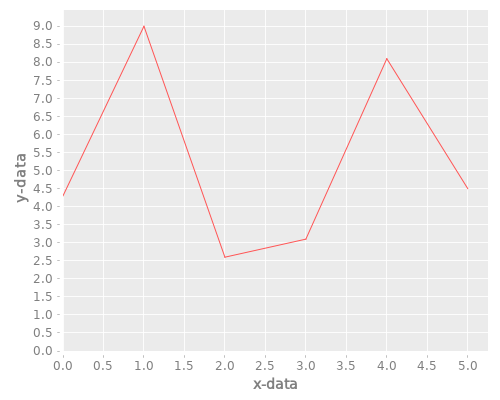
\includegraphics[width=.9\linewidth]{incanter-xy-line.png}
\end{center}

\subsection{OZ}
\label{sec:orga64163d}

From
\url{https://github.com/metasoarous/oz/blob/master/examples/clojupyter-example.ipynb}

\begin{verbatim}
(require '[clojupyter.misc.helper :as helper])
(helper/add-dependencies '[metasoarous/oz "1.6.0-alpha2"])
(require '[oz.notebook.clojupyter :as oz])
\end{verbatim}

\subsubsection{DEFN PLAY DATA}
\label{sec:org18b2e55}

\begin{verbatim}
(do (defn play-data [& names]
      (for [n names
            i (range 20)]
        {:time i :item n :quantity (+ (Math/pow (* i (count n)) 0.8) (rand-int (count n)))}))

    (def stacked-bar
      {:data {:values (play-data "munchkin" "witch" "dog" "lion" "tiger" "bear")}
       :mark "bar"
       :encoding {:x {:field "time"}
                  :y {:aggregate "sum"
                      :field "quantity"
                      :type "quantitative"}
                  :color {:field "item"}}})
    (oz/view! stacked-bar)   )
\end{verbatim}

\begin{verbatim}
class clojure.lang.Compiler$CompilerExceptionclass clojure.lang.Compiler$CompilerExceptionSyntax error compiling at (composable-statistics:localhost:34413(clj)*:15:5).
No such namespace: oz
\end{verbatim}


\begin{verbatim}
;; Create spec, then visualize
(def spec
  {:data {:url "https://gist.githubusercontent.com/metasoarous/4e6f781d353322a44b9cd3e4597c532c/raw/cd633d9bb8e0bed4a5b8e66a32b9569ca2147989/cars.json"}
   :mark "point"
   :encoding {
     :x {:field "Horsepower", :type "quantitative"}
     :y {:field "Miles_per_Gallon", :type "quantitative"}
     :color {:field "Origin", :type "nominal"}}})
(oz/view! spec)
\end{verbatim}

\begin{verbatim}
#'composable-statistics.core/specclass clojure.lang.Compiler$CompilerExceptionclass clojure.lang.Compiler$CompilerExceptionSyntax error compiling at (composable-statistics:localhost:34413(clj)*:10:1).
No such namespace: oz
\end{verbatim}


\begin{verbatim}
(oz/view!
  [:div
   [:h1 "A little hiccup example"]
   [:p "Try drinking a glass of water with your head upside down"]
   [:div {:style {:display "flex" :flex-direction "row"}}
    [:vega-lite spec]
    [:vega-lite stacked-bar]]])
\end{verbatim}

\begin{verbatim}
class clojure.lang.Compiler$CompilerExceptionclass clojure.lang.Compiler$CompilerExceptionSyntax error compiling at (composable-statistics:localhost:34413(clj)*:2:1).
No such namespace: oz
\end{verbatim}

\section{GAUSSIAN PROCESSES}
\label{gaussian-processes}
The Extended Kalman Filter above is a generalization of linear
regression.

\subsection{RECURRENT LINEAR REGRESSION}
\label{recurrent-linear-regression}
Emacs 26.2 of 2019-04-12, org version: 9.2.2
\end{document}
